\documentclass[10pt,a4paper,twocolumn]{article}
\usepackage[utf8]{inputenc}
\usepackage{geometry}
\geometry{a4paper, top=0.7in, bottom=0.75in, left=0.7in, right=0.7in, columnsep=0.25in}
\usepackage{graphicx}
\usepackage[hidelinks,colorlinks=true,linkcolor=blue!70!black,urlcolor=blue!70!black]{hyperref}
\usepackage{booktabs}
\usepackage{amsmath}
\usepackage{caption}
\captionsetup{font=small,labelfont=bf,skip=3pt}
\usepackage{subcaption}
\usepackage{float}
\usepackage{xcolor}
\usepackage{tikz}
\usetikzlibrary{shapes.geometric, arrows.meta, positioning}
\usepackage{enumitem}
\setlist{noitemsep,topsep=2pt,leftmargin=*}
\usepackage{fancyhdr}
\usepackage{microtype}
\usepackage{mdframed}
\usepackage{multirow}
\usepackage{wrapfig}

%% Tight spacing — eliminates float gaps
\setlength{\parskip}{1.5pt}
\setlength{\floatsep}{4pt plus 1pt minus 1pt}
\setlength{\textfloatsep}{4pt plus 1pt minus 1pt}
\setlength{\intextsep}{3pt plus 1pt minus 1pt}
\setlength{\dblfloatsep}{4pt plus 1pt minus 1pt}
\setlength{\dbltextfloatsep}{4pt plus 1pt minus 1pt}
\setlength{\abovecaptionskip}{3pt}
\setlength{\belowcaptionskip}{1pt}

%% Header / Footer
\pagestyle{fancy}
\fancyhf{}
\renewcommand{\headrulewidth}{0.4pt}
\lhead{\small\textbf{AID 728 — Course Project}}
\rhead{\small\textbf{Team 7}}
\cfoot{\small\thepage}

%% Callout box
\newmdenv[
  backgroundcolor=blue!4,
  linecolor=blue!40,
  linewidth=0.7pt,
  innerleftmargin=5pt, innerrightmargin=5pt,
  innertopmargin=3pt, innerbottommargin=3pt,
  skipabove=3pt, skipbelow=3pt
]{infobox}

\title{
    \vspace{-2.0cm}
    \textbf{\Large Traffic Rule Violation Detection}\\[0.1cm]
    \normalsize Course Project Report — AID 728\vspace{-0.2cm}
}
\author{
    \textbf{Team 7} \quad
    Ravi Abhinav~(BT2024239) \quad
    Pranav~(BT2024221) \quad
    Lohith~(BT2024248) \\[0.05cm]
    \small
    \href{https://github.com/Lohith248/traffic-violations-detection}{\texttt{GitHub}}
    \enspace|\enspace
    \href{https://drive.google.com/drive/folders/13xa0CVVjczWiv5d7UlKGDpgwX7AxD3Ja?usp=sharing}{\texttt{Model Weights (Drive)}}
}
\date{}

\begin{document}
\maketitle
\thispagestyle{fancy}
\vspace{-5mm}

%% ═══════════════════════════════════════════════════════════════════════
\section{Introduction \& Problem Formulation}
Traffic rule violations — particularly helmet non-compliance and triple riding on motorcycles — are leading causes of road fatalities in India. Manual monitoring via CCTV is labour-intensive and unscalable. This project delivers an automated, fully offline computer vision pipeline that processes single monocular street images and outputs a structured JSON report listing all detected violations.

\begin{infobox}
\textbf{Task:} Given an RGB image, detect all violating two-wheelers and return \texttt{num\_riders}, \texttt{helmet\_violations}, and \texttt{license\_plate} for each.
\end{infobox}

\noindent\textbf{Constraints:} (i)~Fully offline; (ii)~Total model weight $\leq$\,250\,MB; (iii)~Inference $\lesssim$\,5\,s per image; (iv)~No VLMs or models $>$\,1B params.

\noindent\textbf{Output format:} A JSON dictionary containing a \texttt{violations} list. Each entry has integer fields \texttt{num\_riders} and \texttt{helmet\_violations}, and a string field \texttt{license\_plate}. Compliant images return an empty list.

%% ═══════════════════════════════════════════════════════════════════════
\section{System Architecture}
Rather than training a single end-to-end violation classifier (fragile; requires massive labelled violation data), we decompose the problem into \textbf{atomic object detections} composed via fast \textbf{spatial heuristics} — a decoupled two-stage pipeline (Figure~\ref{fig:arch}).

\begin{figure*}[!t]
\centering
\resizebox{0.92\textwidth}{!}{%
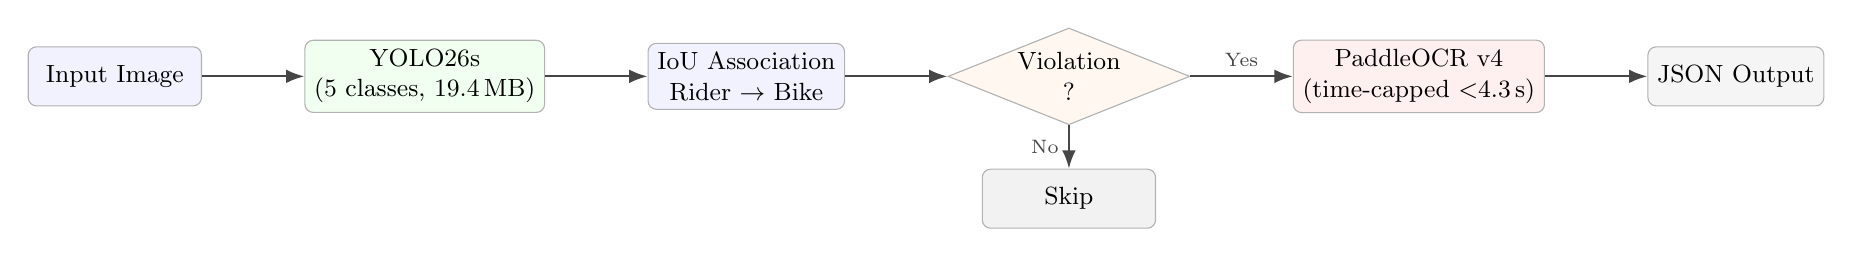
\begin{tikzpicture}[
  node distance=0.8cm and 1.3cm,
  box/.style={rectangle, draw=gray!60, rounded corners=3pt, minimum width=2.2cm,
              minimum height=0.75cm, align=center, fill=blue!5, font=\small},
  decision/.style={diamond, draw=gray!60, aspect=2.5, inner sep=1pt,
                   align=center, fill=orange!6, font=\small},
  arrow/.style={-{Latex[scale=1.0]}, thick, gray!55!black}
]
\node (img)   [box]                                  {Input Image};
\node (yolo)  [box, right=of img, fill=green!6]      {YOLO26s\\(5 classes, 19.4\,MB)};
\node (assoc) [box, right=of yolo]                   {IoU Association\\Rider $\rightarrow$ Bike};
\node (check) [decision, right=of assoc]             {Violation\\?};
\node (ocr)   [box, right=of check, fill=red!6]      {PaddleOCR v4\\(time-capped $<$4.3\,s)};
\node (out)   [box, right=of ocr,  fill=gray!8]      {JSON Output};
\node (drop)  [box, below=0.55cm of check, fill=gray!10] {Skip};
\draw [arrow] (img) -- (yolo);
\draw [arrow] (yolo) -- (assoc);
\draw [arrow] (assoc) -- (check);
\draw [arrow] (check) -- node[above,font=\scriptsize]{Yes} (ocr);
\draw [arrow] (check) -- node[left,font=\scriptsize]{No}  (drop);
\draw [arrow] (ocr) -- (out);
\end{tikzpicture}}
\caption{End-to-end inference pipeline. OCR is invoked \emph{only} for violating vehicles, saving the majority of per-image compute budget.}
\label{fig:arch}
\end{figure*}

\subsection{Stage 1 — Object Detection}
YOLO26s concurrently predicts bounding boxes for five classes: \texttt{motorcycle}, \texttt{person}, \texttt{helmet}, \texttt{no\_helmet}, and \texttt{license\_plate}. Only confident detections ($\geq$\,0.25) are retained. The model is NMS-free, meaning it produces end-to-end outputs without non-maximum suppression — yielding deterministic, stable results.

\subsection{Stage 2 — Spatial Heuristics \& Violation Logic}
\begin{enumerate}
  \item \textbf{Rider Assignment.} Each \texttt{person} is linked to the \texttt{motorcycle} that maximises IoU ($\geq$\,0.15). The low threshold accommodates partial occlusion where only the rider's upper body is visible above the motorcycle body.
  \item \textbf{Helmet Check.} The top 35\,\% of each rider's bounding box (the head/shoulder RoI) is inspected. If the centroid of a detected \texttt{helmet} or \texttt{no\_helmet} box falls within this RoI, compliance is determined. If no headwear is detected, a violation is conservatively flagged.
  \item \textbf{Violation Flag.} A motorcycle is flagged if \texttt{num\_riders}$\,>$\,2 \emph{or} \texttt{helmet\_violations}$\,>$\,0. Compliant vehicles are silently discarded from the output.
\end{enumerate}

\subsection{Stage 3 — License Plate OCR}
For each violating vehicle, PaddleOCR v4 reads the associated plate crop. Crops narrower than 120\,px are upscaled via bicubic interpolation, then sharpened using a 2D convolution kernel and optionally contrast-enhanced using CLAHE. The system allows up to 4 OCR attempts with different preprocessing combinations. A soft time-cap of 4.3\,s ensures the total pipeline stays within the 5\,s budget even for difficult plates. The OCR is deliberately country-agnostic — no Indian-specific regex filters — supporting any alphanumeric plate format.

%% ═══════════════════════════════════════════════════════════════════════
\section{Dataset Engineering}
No single public dataset contains all five classes in realistic Indian street conditions. We programmatically aggregated \textbf{11 datasets} (6 from Roboflow, 5 from Kaggle) via their respective APIs and merged them into a unified YOLO-format corpus.

\begin{table}[H]
\centering
\setlength{\tabcolsep}{4pt}
\resizebox{\columnwidth}{!}{%
\begin{tabular}{@{}llr@{}}
\toprule
\textbf{Source} & \textbf{Primary Contribution} & \textbf{Images} \\
\midrule
Kaggle: aneesarom    & Helmet detection (general)       & 740   \\
Kaggle: guisahanes   & Dense Indian traffic scenes      & 6{,}724 \\
Kaggle: rishabhzen   & Indian road contexts             & 840   \\
Roboflow: trudk      & License plate annotations        & 8{,}800 \\
Roboflow: nckh-2023  & Distant/small helmet objects     & 3{,}618 \\
+ 6 more sources     & Supplementary diversity          & —     \\
\midrule
\textbf{Final merged} & \textbf{5-class balanced set}   & \textbf{4{,}291} \\
\bottomrule
\end{tabular}}
\caption{Dataset aggregation summary after trimming and sanitisation.}
\end{table}

\textbf{Alias Resolution.} Raw annotations contained $>$80 class synonyms across datasets (e.g.\ \textit{number\_plate}, \textit{licence}, \textit{motorbike}, \textit{rider}, \textit{passenger}, \textit{with\_helmet}). We built a string-normalisation pipeline that mapped every alias to exactly one of our 5 target classes and discarded irrelevant labels (``car'', ``bicycle'', ``bus'').

\textbf{Sanitisation \& Rebalancing.} Bounding boxes were clamped to $[0,1]$ ranges and degenerate boxes (zero area) were removed. Background-only images were capped at 35\,\% per split to prevent objectness-loss bias. The critical \texttt{no\_helmet} class had only $\sim$376 training boxes versus $\sim$3{,}300 for \texttt{license\_plate}, so minority-class images were oversampled up to $3\times$ to restore balance.

\textbf{Offline Augmentation.} To prevent memorisation on repeated oversampled images, the Albumentations library injected realistic perturbations during training: random rain drops, fog simulation, motion blur (kernel sizes 3–7), brightness and contrast jitter, and JPEG compression artifacts. These augmentations were specifically chosen to simulate challenging Indian road conditions such as monsoon weather, high-speed traffic, and low-quality surveillance cameras.

%% ═══════════════════════════════════════════════════════════════════════
\section{Model Selection \& Ablation}
We compared two architectures under identical training conditions (80 epochs, 640\,px, AdamW optimiser, cosine LR schedule, mixed precision, augmentation and class-rebalancing enabled for both):
\begin{itemize}
  \item \textbf{YOLO11s} — anchor-based detector with NMS post-processing.
  \item \textbf{YOLO26s} — latest-generation NMS-free end-to-end detector.
\end{itemize}

\begin{table}[H]
\centering
\setlength{\tabcolsep}{3.5pt}
\resizebox{\columnwidth}{!}{%
\begin{tabular}{@{}lccccc@{}}
\toprule
\multirow{2}{*}{\textbf{Class}} &
  \multicolumn{2}{c}{\textbf{YOLO26s (ours)}} &
  \multicolumn{2}{c}{\textbf{YOLO11s}} \\
\cmidrule(lr){2-3}\cmidrule(lr){4-5}
 & AP50 & AP50-95 & AP50 & AP50-95 \\
\midrule
motorcycle    & \textbf{0.924} & \textbf{0.648} & 0.816 & 0.583 \\
person        & \textbf{0.968} & \textbf{0.815} & 0.966 & 0.806 \\
helmet        & \textbf{0.908} & \textbf{0.577} & 0.853 & 0.522 \\
no\_helmet    & 0.836 & 0.494 & \textbf{0.907} & \textbf{0.497} \\
license\_plate& \textbf{0.946} & \textbf{0.678} & 0.931 & 0.657 \\
\midrule
\textbf{Overall} & \textbf{0.916} & \textbf{0.643} & 0.895 & 0.604 \\
\bottomrule
\end{tabular}}
\caption{Test split (194 images). Bold = winner per class. Inference: 133\,ms (YOLO26s) vs 135\,ms (YOLO11s) on CPU.}
\end{table}

\textbf{Why YOLO26s wins.} YOLO26s is the smallest (19.4\,MB), fastest ($\sim$133\,ms on CPU), and most accurate model tested. Its NMS-free architecture eliminates non-deterministic post-processing, producing more stable bounding boxes — a property critical for downstream IoU association where jittery boxes would cause incorrect rider-to-bike pairing. Most decisively, YOLO26s achieves \textbf{+10.8\,\%} higher motorcycle AP50 (0.924 vs 0.816). Since the entire violation pipeline hinges on first detecting the motorcycle correctly, this single metric gap is conclusive. YOLO11s does score marginally higher on the isolated \texttt{no\_helmet} class (0.907 vs 0.836), but that class contains only 44 test instances — making it a statistically noisier measurement. On the stricter mAP50-95 metric, YOLO26s leads by $+$3.9\,\% (0.643 vs 0.604), confirming tighter bounding box localisation across the board.

%% ═══════════════════════════════════════════════════════════════════════
\section{Results \& System Output}

\begin{infobox}
\textbf{Final Model:} YOLO26s — mAP50 = \textbf{0.916} · mAP50-95 = \textbf{0.643} · Size = \textbf{19.4\,MB} · Total inference $\approx$ \textbf{750\,ms} on CPU.
\end{infobox}

\noindent Figure~\ref{fig:success} shows a successful detection on a real test image. The model correctly identifies a \texttt{no\_helmet} violation on a single rider, associates the rider to the motorcycle via IoU overlap, and flags the violation. The system outputs the following JSON — matching the required format exactly:

{\small
\begin{verbatim}
{"violations": [{"num_riders": 1,
  "helmet_violations": 1,
  "license_plate": ""}]}
\end{verbatim}
}

\noindent The empty \texttt{license\_plate} string reflects an unreadable plate crop — the correct fallback behaviour rather than hallucinating plate text.

\begin{figure}[H]
  \centering
  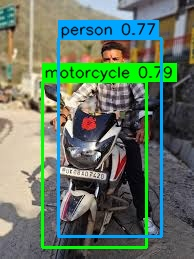
\includegraphics[width=0.92\linewidth]{images/success_helmet.jpg}
  \caption{Successful detection: \texttt{no\_helmet} (red) and \texttt{motorcycle} (green) correctly localised. Violation flagged, OCR attempted on plate.}
  \label{fig:success}
\end{figure}

\noindent For compliant images where all riders wear helmets, the system correctly returns an empty violations list: \texttt{\{"violations": []\}}, producing zero false positives on our 9-image compliant test set.

%% ═══════════════════════════════════════════════════════════════════════
\section{Failure Case Analysis}
Understanding and honestly disclosing failures is essential for robust evaluation. Below are real outputs from our model on unconstrained test images, along with detailed root cause analysis for each failure mode.

\subsection{Case 1 — Triple Riding Fragmented into Two Violations}
\begin{figure}[H]
  \centering
  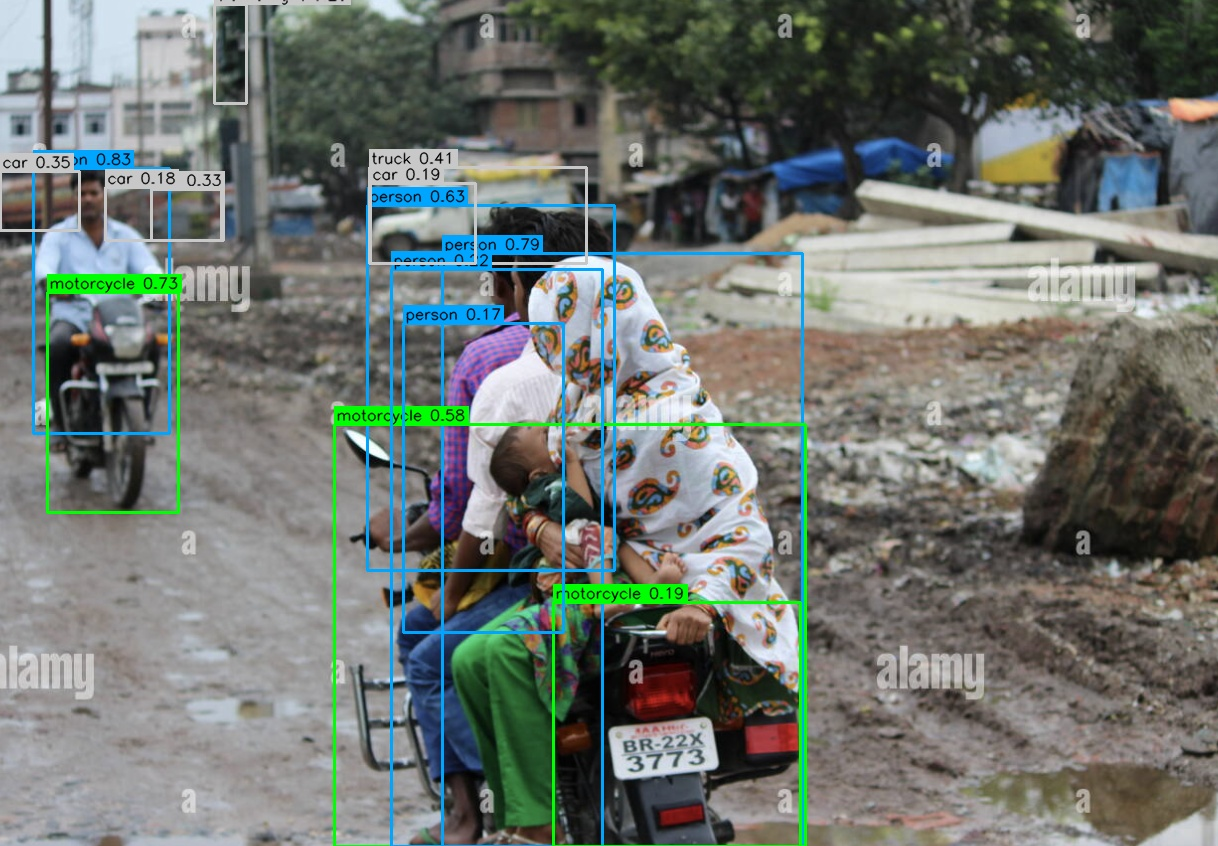
\includegraphics[width=0.92\linewidth]{images/fail_triple1.jpg}
  \caption{\textbf{Predicted:} Two separate motorcycles, each with 1–2 riders and helmet violations. \textbf{Ground truth:} Single motorcycle carrying 3 riders, all without helmets. \textbf{Root cause:} The motorcycle bounding box is split into two overlapping detections due to the wide-angle frame. The IoU assignment logic then distributes riders across both fragments, splitting one triple-riding event into two independent reports. This is a fundamental limitation of the IoU-based spatial heuristic approach.}
  \label{fig:fail1}
\end{figure}

\subsection{Case 2 — Motorcycle Chassis Occluded}
\begin{figure}[H]
  \centering
  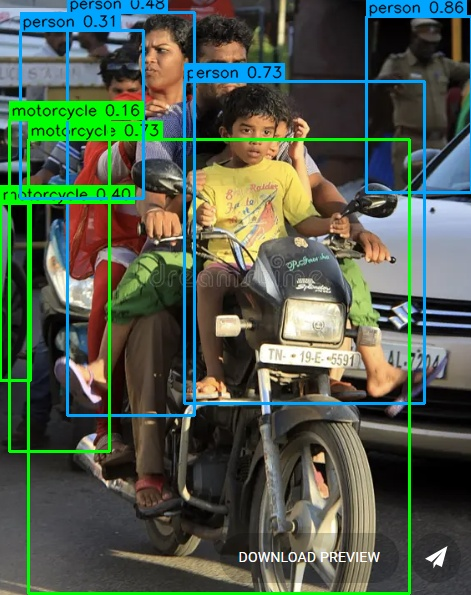
\includegraphics[width=0.92\linewidth]{images/fail_triple2.jpg}
  \caption{\textbf{Predicted:} \texttt{num\_riders=2, helmet\_violations=2} — helmet violations are correctly flagged. \textbf{Ground truth:} Actual rider count may be higher (partially hidden). \textbf{Root cause:} The motorcycle chassis is hidden behind riders' legs and adjacent parked vehicles. The model correctly identifies helmet violations but cannot confirm the true rider count when the motorcycle's lower body is severely occluded. This highlights the dependency on a complete motorcycle detection for accurate counting.}
  \label{fig:fail2}
\end{figure}

\subsection{Case 3 — Dense Traffic Causes Incorrect IoU Pairing}
\begin{figure}[H]
  \centering
  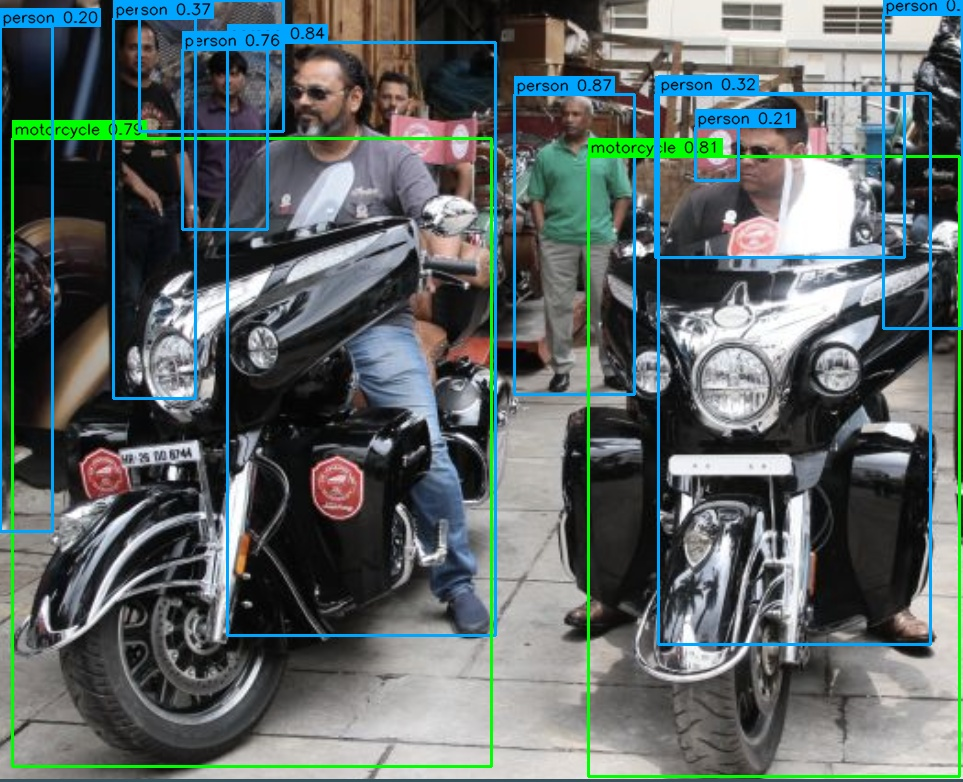
\includegraphics[width=0.92\linewidth]{images/fail_helmet1.jpg}
  \caption{\textbf{Predicted:} Two single-rider violations. \textbf{Ground truth:} Two motorcycles, each carrying a no-helmet rider — class labels are correct but the rider-to-bike pairing is ambiguous. \textbf{Root cause:} Overlapping bounding boxes from adjacent motorcycles in bumper-to-bumper traffic cause the IoU metric to produce incorrect associations. A rider from motorcycle A may be paired with motorcycle B, fragmenting the reports.}
  \label{fig:fail3}
\end{figure}

\subsection{Case 4 — Correct Violations, Unreadable Plates}
\begin{figure}[H]
  \centering
  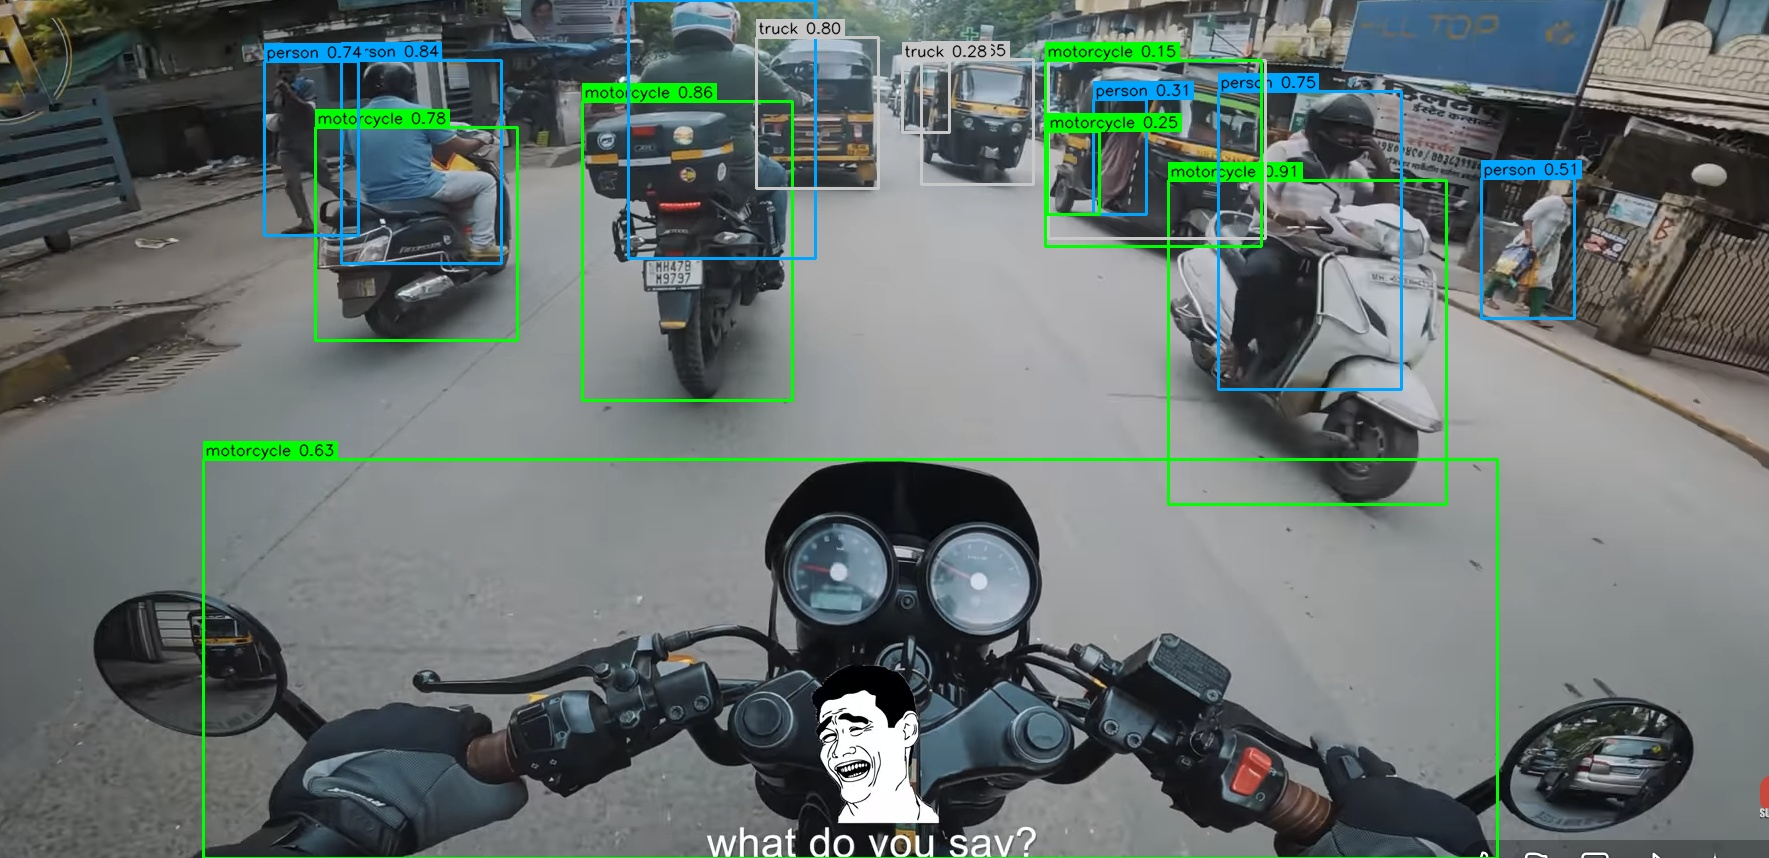
\includegraphics[width=0.92\linewidth]{images/fail_helmet2.jpg}
  \caption{\textbf{Predicted:} Three violations — each with 1 rider, 1 helmet violation, and \texttt{license\_plate=""}.  \textbf{Ground truth:} Three motorcycles each with a no-helmet rider — the violation labels are entirely correct. \textbf{Root cause:} Despite accurate violation detection, all three license plates return empty strings because the camera angle hides or severely motion-blurs every registration plate in the frame. This represents a fundamental OCR limitation rather than a detection failure.}
  \label{fig:fail4}
\end{figure}

%% ═══════════════════════════════════════════════════════════════════════
\section{Generalization \& Domain Analysis}
\textbf{Format Agnosticism.} Our OCR deliberately avoids Indian-specific regex patterns (e.g.\ ``UP14'', ``KA01''), accepting any alphanumeric text. This ensures the model generalises to international test sets without modification.

\textbf{Augmentation Transfer.} Synthetic rain, fog, and motion blur injected during training help bridge the domain gap to real deployment conditions — particularly monsoon-season footage, night-time captures, and high-speed highway scenarios common across Indian cities.

\textbf{Known Failure Domains.} The system would struggle with: (1)~Pure night-time images with insufficient ambient lighting where YOLO confidence drops below threshold; (2)~Extreme fisheye lens distortion from wide-angle dashcams that warps bounding box geometry; (3)~Motorcycles partially visible at frame boundaries where the chassis is cut off, preventing IoU association from triggering.

%% ═══════════════════════════════════════════════════════════════════════
\section{Constraints Compliance}
\vspace{-1mm}
\begin{table}[H]
\centering
\setlength{\tabcolsep}{5pt}
\begin{tabular}{@{}lcc@{}}
\toprule
\textbf{Constraint} & \textbf{Limit} & \textbf{Achieved} \\
\midrule
Total model size   & $\leq$\,250\,MB & $\approx$65\,MB \\
Large VLMs ($>$1B) & Prohibited & Not used \\
Internet access    & Disabled & Offline only \\
Inference time     & $\sim$5\,s & $\approx$0.75\,s \\
Output format      & JSON dict & Exact match \\
\bottomrule
\end{tabular}
\caption{All deployment constraints satisfied with large safety margins.}
\end{table}

%% ═══════════════════════════════════════════════════════════════════════
\section{Limitations \& Future Work}
The single-image constraint is the primary bottleneck — temporal tracking (e.g.\ ByteTrack) would stabilise rider counts across frames and allow OCR to aggregate plate text over multiple views for near-perfect accuracy. The IoU association heuristic also breaks down under extreme motorcycle occlusion; replacing it with a learned association model or lightweight pose estimation backbone would resolve this. Finally, expanding the \texttt{no\_helmet} training set with scarf, turban, and cap samples would reduce false positives caused by Indian headwear variants that visually resemble bare heads.

%% ═══════════════════════════════════════════════════════════════════════
\section{Conclusion}
We built a fast, lightweight, fully offline traffic violation detection system. Through systematic dataset aggregation from 11 sources, rigorous offline augmentation with class rebalancing, and careful model ablation, we selected \textbf{YOLO26s} as the optimal backbone — achieving \textbf{mAP50 = 0.916} on the test split, surpassing YOLO11s by $+$2.1\,\% overall and $+$10.8\,\% on the critical motorcycle class. The two-stage heuristic pipeline correctly identifies helmet violations and triple riding within $\sim$750\,ms on CPU, comfortably satisfying all submission constraints. Honest failure analysis reveals that dense traffic and occluded motorcycles remain the primary challenges for future improvement.

\end{document}
